%&"../ai"
\endofdump
\tikzexternalize[prefix=cache/]{project1}
\begin{document}
    \title{项目一:MSA}
    \maketitle
    % 1)对算法的描述以及算法实现结果分析;
    % 2)不同算法的搜索结果;
    % 3)不同算法的运行时间;
    % 4)复杂度分析。

    \tableofcontents
    \clearpage

    \section{题目}

    \subsection{Topic}

    Implement three algorithms to solve multiple sequence alignment (MSA) problems.

    \subsection{Requirements}

    \begin{enumerate}
        \item Implement dynamic programming (DP) algorithm to find the optimal solution.
        \item Implement A-star (A$^\ast$) algorithm to find the optimal solution.
        \item Implement genetic algorithm to find the optimal/suboptimal solution.
    \end{enumerate}

    \subsection{Rules}

    \begin{table}[H]
        \centering
        \caption{Cost Matrix}\label{tab:costmat}
        \begin{tabular}{cccc}
            \toprule
                & Match $\alpha(p,p)$ & Mismatch $\alpha(p,q)$ & Gap $\delta$ \\
            \midrule
            Cost & 0 & 3 & 2 \\
            \bottomrule
        \end{tabular}
    \end{table}

    The table above shows the pairwise cost matrix. For multiple sequence alignment, the cost should be calculated in a cycle pairwise manner. Note that GAP-GAP is a match and should be considered as 0 cost. For every query, find the best alignment(s) in the database with the lowest cost.

    \section{动态规划算法}

    \subsection{双序列比对}

    在算法与复杂性课程\cite{algcom}里,已经提到了双序列比对的动态规划算法,如图 \ref{fig:pairwisedp} 所示,双序列比对对于一个状态只需要考虑三个临近状态的转移,分别是对齐$\alpha$,间隔 $\delta_x$、$\delta_y$,转换行动如表 \ref{tab:pairwise} 所示。对于每一个状态,都需要考虑经过哪一条路径消耗最小,于是就有了如算法 \ref{alg:pairwise} 的动态规划状态转移方程。

    \begin{algorithm}[H]
        \caption{双序列比对动态规划 MSA}\label{alg:pairwise}
        \KwIn{$x_1x_2\cdots x_m, y_1y_2\cdots y_n,\alpha,\delta$}
        \KwOut{最小损耗}
        \BlankLine
        \lFor{$i\leftarrow 0$ to $m$}{$M[i,0]=i\delta$}
        \lFor{$j\leftarrow 0$ to $n$}{$M[0,j]=j\delta$}
        \For{$i\leftarrow 1$ to $m$}{
            \For{$j\leftarrow 1$ to $n$}{
                $M[i,j]=\min(\alpha[x_i,y_j] + M[i-1,j-1], \delta + M[i-1,j], \delta + M[i,j-1])$\;
            }
        }
        \Return{$M[m,n]$}\;
    \end{algorithm}

    \begin{minipage}{0.48\textwidth}
        \begin{table}[H]
            \centering
            \caption{双序列行动坐标变换表}\label{tab:pairwise}
            \begin{tabular}{crr}
                \toprule
                    & $i$ & $j$ \\
                \midrule
                $\alpha$ & $+1$ & $+1$ \\
                $\delta_x$ & $0$ & $+1$ \\
                $\delta_y$ & $+1$ & $0$ \\
                \bottomrule
            \end{tabular}
        \end{table}
    \end{minipage}\hfil
    \begin{minipage}{0.48\textwidth}
        \begin{figure}[H]
            \centering
            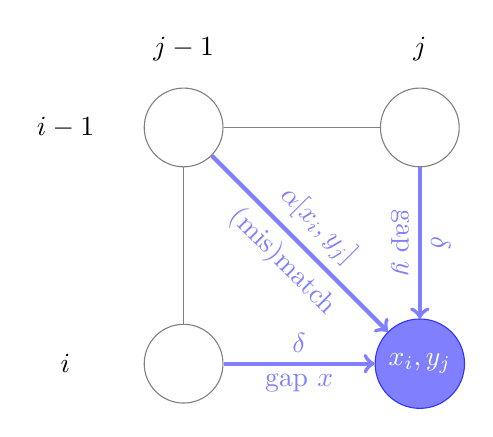
\begin{tikzpicture}
\tikzstyle{strnode}=[circle,draw=gray,minimum width=1cm];
\tikzstyle{move}=[line width=1.5pt, blue!50, ->];
\node[strnode] (v1) at (-1,0.5) {};
\node [strnode] (v3) at (2,0.5) {};
\node [strnode] (v4) at (-1,-2.5) {};
\node [strnode,fill=blue!50,draw=blue!80,font=\color{white}\bfseries] (v2) at (2,-2.5) {$x_i,y_j$};
\draw [move] (v1) edge node[sloped,above] {$\alpha[x_i,y_j]$} node[sloped,below] {(mis)match} (v2);
\draw [move] (v3) edge node[sloped,above] {$\delta$} node[sloped,below] {gap $y$} (v2);
\draw [move] (v4) edge node[sloped,above] {$\delta$} node[sloped,below] {gap $x$} (v2);
\draw[gray] (v1) edge (v3);
\draw[gray] (v1) edge (v4);
\node at (-2.5,0.5) {$i-1$};
\node at (-2.5,-2.5) {$i$};
\node at (2,1.5) {$j$};
\node at (-1,1.5) {$j-1$};
\end{tikzpicture}
            \caption{双序列比对}\label{fig:pairwisedp}
        \end{figure}
    \end{minipage}
    \medskip
    
    \subsection{多序列比对}

    对于三序列比对,情况就复杂地多,需要同时考虑七条路径。

    \begin{minipage}{0.48\textwidth}
        \begin{table}[H]
            \centering
            \caption{三序列行动坐标变换表}\label{tab:multiple}
            \begin{tabular}{crrr}
                \toprule
                    & $k$ & $j$ & $i$ \\
                \midrule
                $\alpha_x\delta_y\delta_z$  & 0 & 0 & 1\\
                $\delta_x\alpha_y\delta_z$ & 0 & 1 & 0 \\
                $\delta_x\alpha_y\alpha_z$ & 0 & 1 & 1 \\
                $\delta_x\delta_y\alpha_z$ & 1 & 0 & 0 \\
                $\alpha_x\delta_y\alpha_z$ & 1 & 0 & 1 \\
                $\alpha_x\alpha_y\delta_z$ & 1 & 1 & 0 \\
                $\alpha_x\alpha_y\alpha_z$ & 1 & 1 & 1 \\
                \bottomrule
            \end{tabular}
        \end{table}
    \end{minipage}\hfil
    \begin{minipage}{0.48\textwidth}
        \begin{figure}[H]
            \centering
            \input{fig/multiple_dp.tex}
            \caption{三序列比对}\label{fig:multipledp}
        \end{figure}
    \end{minipage}
    \medskip

    可以统一化为多序列比对问题。对于 $L$ 条序列比对,首先需要递归地初始化低维度边缘(如图 \ref{fig:downdim} 所示),之后余下空间其行动转换方法可以被表示为二进制从 $(\underbrace{0\cdots01}_{L\text{ digits}})_2$ 到 $(\underbrace{1\cdots11}_{L\text{ digits}})_2$ 内所有的数(最低位为第一维度),计算损耗使用上三角成对比较,规则统一为
    \begin{equation*}
        \texttt{compare}=
        \begin{cases}
            0,& (-,-) \| (p,p) \\
            2,& (p,-) \| (-,q) \\
            3,& (p,q)
        \end{cases}
    \end{equation*}
    并在确定每一次行动后记录路径,最后回溯路径到原点。

    \begin{figure}[H]
        \centering
        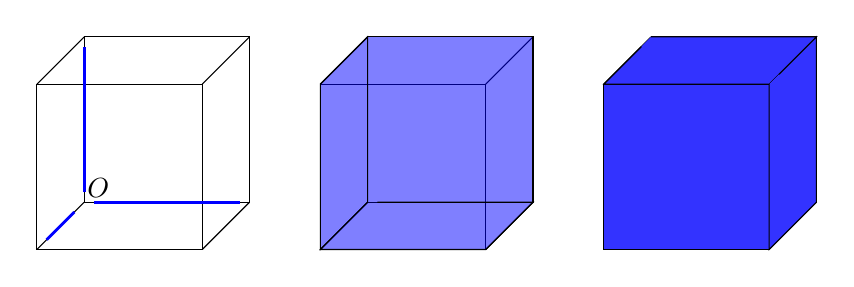
\begin{tikzpicture}[scale=0.6]
\tikzstyle{visited}=[line width=1pt,blue];

\draw  (-2.5,1.5) node (v2) {} rectangle (1,-2) node (v4) {};
\draw  (-1.5,2.5) node (v1) {} rectangle (2,-1) node (v3) {};
\draw (1,1.5) -- (2,2.5);
\draw (-1.5,-1) node (v7) {} -- (-2.5,-2) node (v9) {};
\draw (2,-1) node (v10) {} --  (1,-2);
\draw  (-1.5,2.5) node (v8) {} --  (-2.5,1.5) ;

\draw (7,1.5) -- (8,2.5);
\draw (4.5,-1) node (v11) {} -- (3.5,-2) node (v12) {};
\draw (8,-1) --  (7,-2);
\draw  (4.5,2.5) node (v6) {} --  (3.5,1.5) node (v5) {} ;
\draw  (v5) rectangle (7,-2) node (v15) {};
\draw [fill=blue,fill opacity=0.5] (v6) rectangle (8,-1) node (v16) {};
\draw [fill=blue,fill opacity=0.5] (4.5,2.5) --  (4.5,-1) node (v13) {} -- (3.5,-2) node (v14) {} -- (3.5,1.5) -- cycle;
\draw [fill=blue,fill opacity=0.5] (4.5,-1) -- (3.5,-2) -- (7,-2) -- (8,-1) -- (v13);

\draw (13,1.5) -- (14,2.5) node (v17) {};
\draw (10.5,-1) -- (9.5,-2);
\draw (14,-1) --  (13,-2);
\draw  (10.5,2.5) node (v6) {} --  (9.5,1.5) node (v5) {} ;
\draw  (v6) rectangle (14,-1) node (v20) {};
\draw [fill=blue!80]  (v5) rectangle (13,-2) node (v19) {};

\draw [visited] (v7) edge (v8);
\draw [visited] (v7) edge (v9);
\draw [visited] (v7) edge (v10);

\draw[fill=blue!80] (v6) -- (9.5,1.5) -- (13,1.5) node (v18) {} -- (14,2.5) node (v21) {} -- (10.5,2.5);

\draw[fill=blue!80] (13,1.5) -- (13,-2) --  (14,-1)  --(14,2.5)-- (v18);
\node at (-1.2,-0.7) {$O$};
\end{tikzpicture}
        \caption{降维递归}\label{fig:downdim}
    \end{figure}

    % 29s
    % > 24h
    % 8 核多线程进行中

    几乎类似于双序列比对,下面是 \verb"numpy" 实现版本,虽然其速度没有使用 Python 内置的 \verb"list" 版本(\href{./msa\_mdp.py}{\ttfamily msa\_mdp.py})的快,但是代码可读性已经与伪代码相当。

    \codeseg[language=python]{msa\_ndp.py}{44}{86}

    \subsection{运行时间}

    如果字符串平均长度为 $l$,该算法 $L$ 维字符串的复杂度为:
    \begin{equation*}
        O_S = \prod_{i=1}^L \texttt{len}(S[i]) \approx l^L
    \end{equation*}

    对于该问题,有 $m$ 个待比对序列,$n$ 个数据库项目,总时间复杂度为:
    \begin{equation*}
        mC_{n}^{L-1}O_S \approx mC_{n}^{L-1}l^L
    \end{equation*}

    实际运行时间如表 \ref{tab:dp},在服务器上运行时间如下。

    \begin{table}[h]
        \centering
        \caption{动态规划运行时间}\label{tab:dp}
        \begin{tabular}{cb{3cm}b{3cm}b{3cm}b{3cm}}
            \toprule
             &\multicolumn{2}{c}{\bfseries 双序列}  &\multicolumn{2}{c}{\bfseries 三序列} \\
             \cmidrule(r){2-3}\cmidrule(r){4-5} 
             & \bfseries 朴素实现 \href{./msa\_dp.py}{\ttfamily msa\_dp.py} &\bfseries \verb"list"实现 \href{./msa\_mdp.py}{\ttfamily msa\_mdp.py} &\bfseries \verb"list" 实现 \href{./msa\_mdp.py}{\ttfamily msa\_mdp.py} &\bfseries \verb"numpy" 实现 \href{./msa\_ndp.py}{\ttfamily msa\_ndp.py} \\
            \midrule
            运行时间 & 29s & 1min & 24h & $\sim$36h \\
            \bottomrule
        \end{tabular}
    \end{table}

    \section{A* 算法}

    使用启发函数 $g(n) = |\texttt{len}(S_1)-\texttt{len}(S_2)|$。

    

    \bibliography{ref}

\end{document}